\begin{definition}[Newton's Second Law]{def:label}
	To calculate the \textbf{net force} that an object is experiencing, use the following equation:

	$$
		\sum{\vec{F}} = m\vec{a}
	$$

	Or using calculus:
	$$
		\sum{\vec{F}} = m\frac{d\vec{v}}{{dt}}
	$$
\end{definition}

\begin{itemize}
	\item Many times, we will be looking at forces in 2D, which means that the net force looks like the following:
	$$
		\sum F = F_x \vec{i} + F_y \vec{j}
	$$
	\item Since net force has two components, we can solve force problems by analyzing each component of the net force independently because \textbf{the horizontal and vertical directions are independent of each other}
\end{itemize}

\begin{definition}[Newton's Second Law in 2D]{def:label}
	To find the net force of an object that is experiencing forces in multiple directions, use the following formulas:

	$$
		\sum F_x = m\vec{a_x}
	$$
	$$
		\sum F_y = m\vec{a_y}
	$$

	Or using calculus:
	$$
		\sum F_x = m\frac{d\vec{v_x}}{dt}
	$$
	$$
		\sum F_y = m\frac{d\vec{v_y}}{dt}
	$$
\end{definition}
\newpage

\section{Common Forces}

There are many common forces that we will talk about in physics:

\begin{itemize}
	\item \textbf{GRAVITY:} Also called the "weight force," this force is the force that an object experiences due to gravity and can be calculated by using $F_g = mg$ where $m$ is the mass of the object and $g$ is the acceleration due to gravity ($9.81\frac{\m}{\s}$ on Earth).
	\begin{itemize}
		\item NOTE: Some people may also refer to this as the "weight force" and use $F_W$ so be careful with notation as well as \textit{consistent} with your notation
	\end{itemize}
	\item \textbf{NORMAL:} The forces that the suface an object rests on. This forces always acts \textit{perpendicular} to the surface the object is resting on.
	\item \textbf{FRICTION:} If an object is on the ground, the frictional force is the force that always acts opposite to the direction of motion (will talk about frictional force in a later section).
	\item \textbf{TENSION:} The force exterted by a string or similar type of object that holds an object in place. No clear cut formula for finding this force, but drawing a free-body diagram and isolating the tension force will allow you to find the magnitude of the tension force. 
	\item \textbf{SPRING:} The force a spring exterts on an object. Can find the magnitude of the force of a spring by using $F_s = -kx$ where $k$ is the spring constant and $x$ is the distance the string was stretched/compressed.
	\item \textbf{AIRDRAG:} The force of air on an object when an object is in free-fall or moving through the air.
	\item \textbf{CENTRIPETAL:} The force that keeps an object moving in a circle.
	\begin{itemize}
		\item We've talked about centripetal acceleration, and if you have acceleration then you have force.
	\end{itemize}
\end{itemize}


\section{Free Body Diagrams (FBD)}

A \textbf{free body diagram} is a visual representation of all of the forces that are acting on a given object. We represent that object with a simple point and draw arrows (in the proper directions) that represent all of the forces that are acting on an object.\\

\begin{center}\textbf{HOW TO DRAW A FREE BODY DIAGRAM:}\end{center}
\begin{enumerate}
	\item Isolate the object of interest
	\item Diagram the forces that act on the object
	\item Sum the forces
\end{enumerate}
\newpage

\begin{problem}
	A block with mass $m$ is sitting on a table. Draw the FBD of the block and calculate the net force that the block experiences.

	\begin{center}
		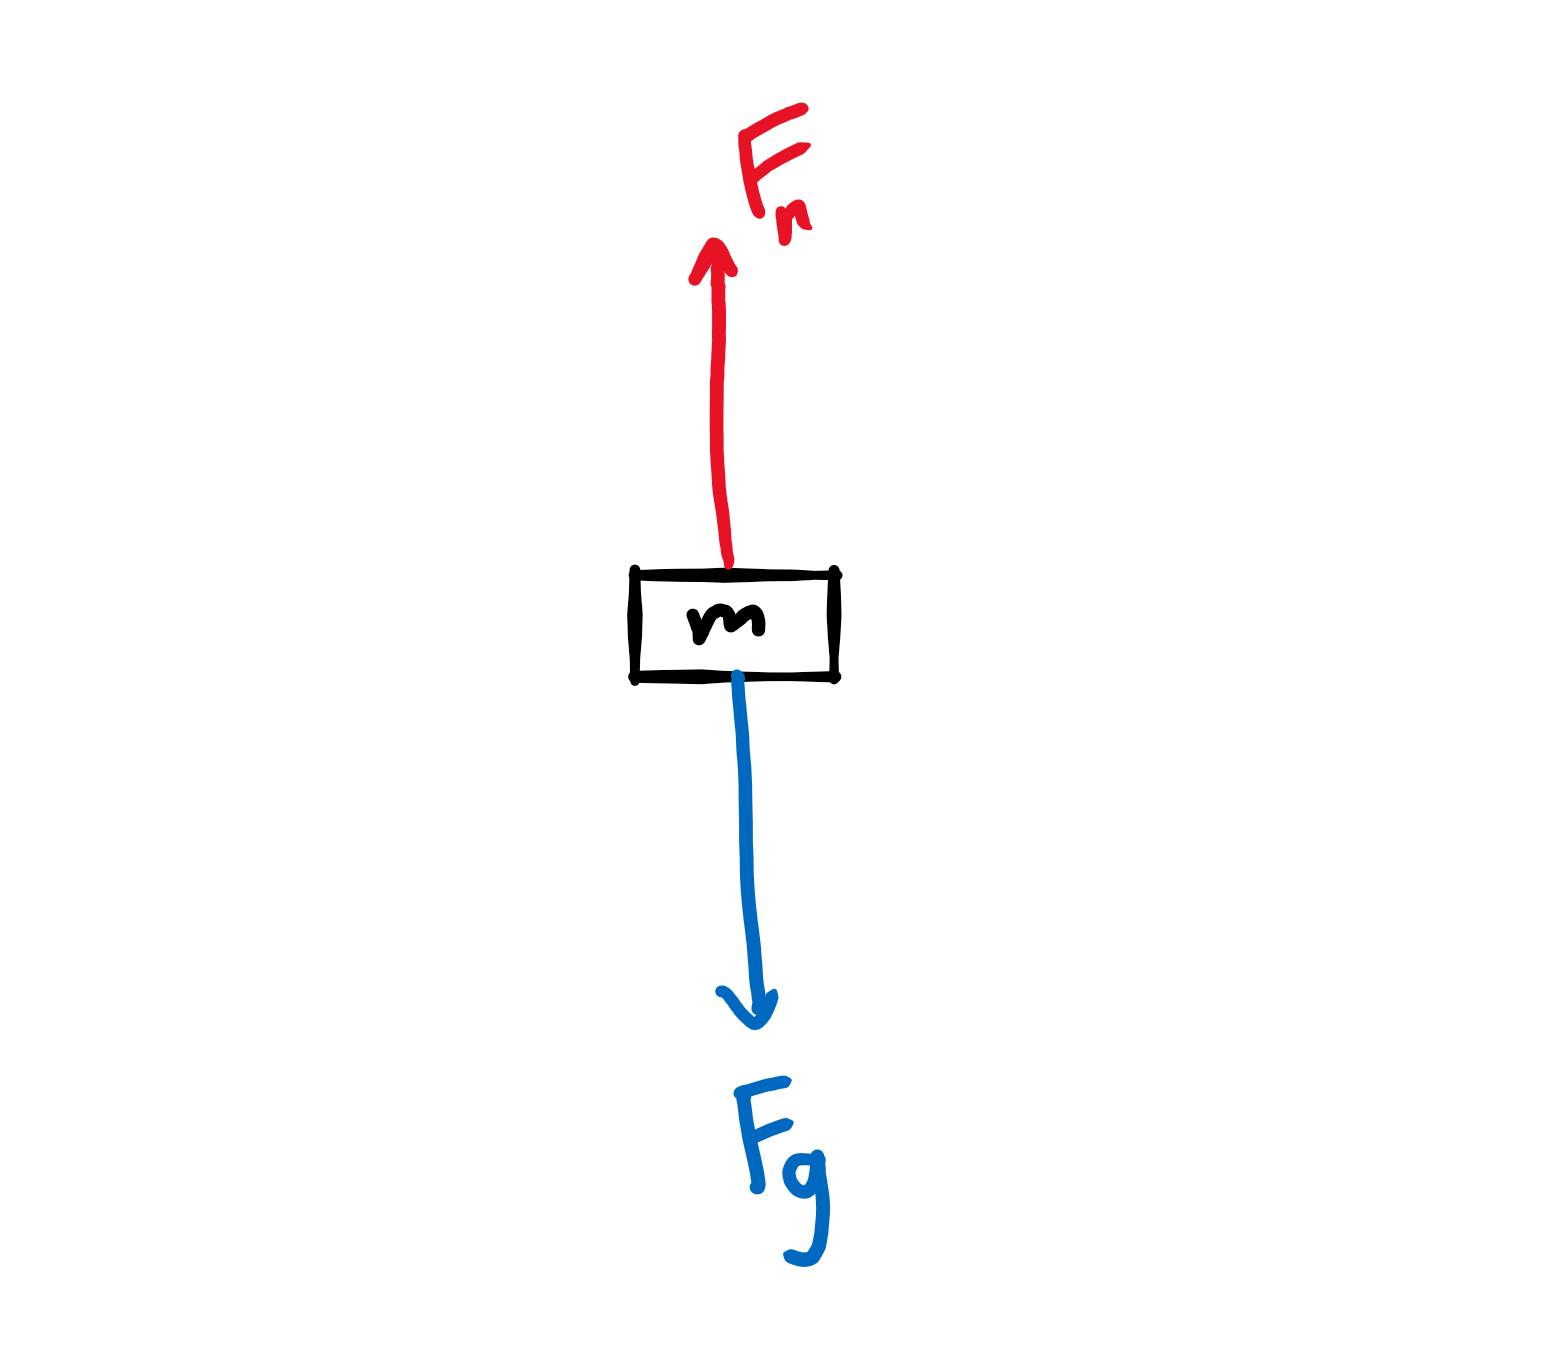
\includegraphics[width=0.5\textwidth]{chapters/ch3/images/fig3_1.PNG}
	\end{center}
	First we can algebraically analyze the forces in the $x$-direction. Since the object is not moving, its acceleration must be 0. There are also no forces being acted on the block in the $x$-direction. Therefore:
	$$
		\begin{aligned}
			\sum F_x = m\vec{a_x} = 0\\
		\end{aligned}
	$$

	Now we can algebraically solve for the net force in the $y$-direction. Since the object is not moving, its acceleration must be 0. Therefore:
	$$
		\begin{aligned}
			\sum F_y = m\vec{a_y} = 0\\
			\sum F_y = F_N - F_g = F_N - mg
		\end{aligned}
	$$

	Threfore, the total net force of the block is as follows:
	$$
		\sum F = 0\vec{i} + F_n-mg \vec{j}
	$$
\end{problem}


\section{Other Posssible Scenarios and Their FBDs}

While many systems are just on the ground, there are many other physical situations where objects are hanging or on an incline. Here are some examples of FBDs of the three common scenarios of objects that are not simply on the ground:

\subsection*{Hanging From a Rope}

\begin{center}
	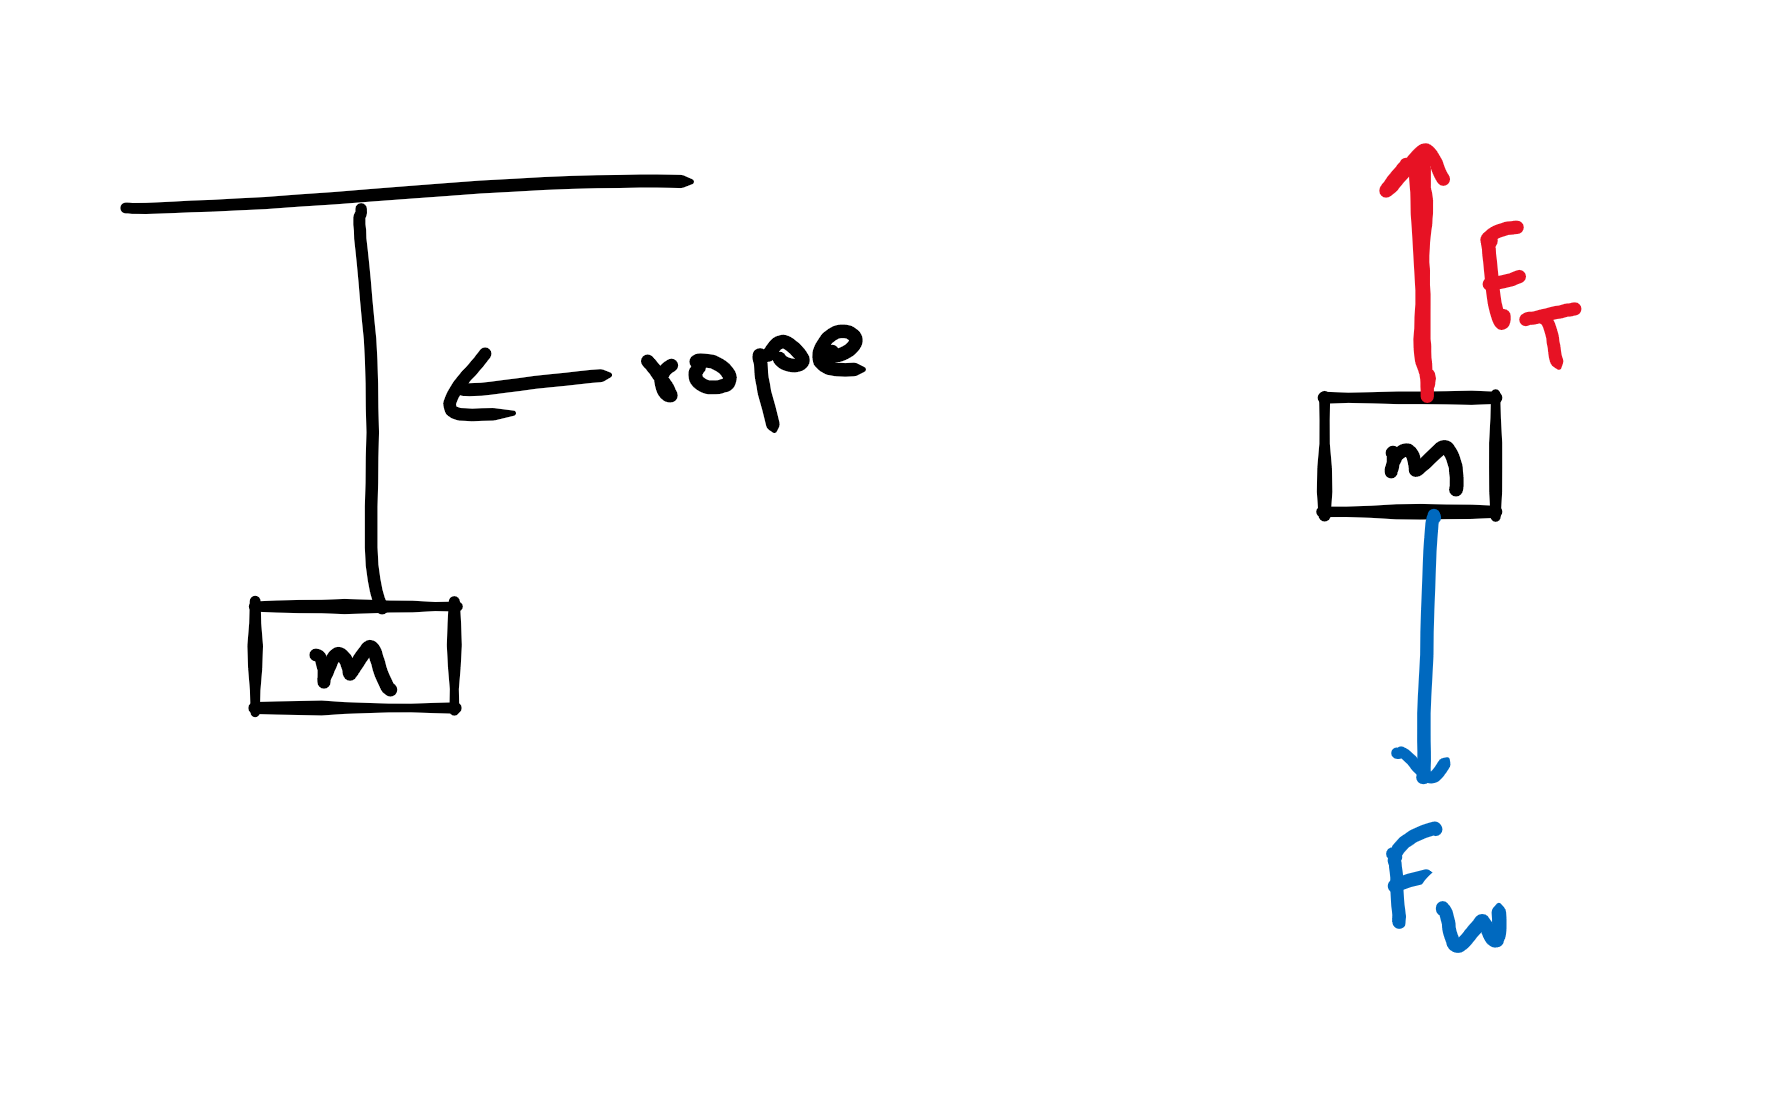
\includegraphics[width=0.5\textwidth]{chapters/ch3/images/fig3_2.PNG}
\end{center}

In the FBD pictured above, notice how there is no normal force because a normal force ony exists if an object is resting on a surface (in this case the object is airborne). We can also solve this algebraically:

$$
	\begin{aligned}
		&\sum F = m\vec{a} = 0 \:\:\:\text{(object is in equilibrium)}\\
		&\sum F_x = 0 \:\:\:\text{(there are no forces in the $x$ direction)}\\
		&\sum F_y = F_T - F_g = F_t - mg
	\end{aligned}
$$

Keep in mind that $F_T$ is the \textit{tension force}, which is the force that the rope pulls on the object that it is attached to.

\subsection*{On a Pulley}

\begin{center}
	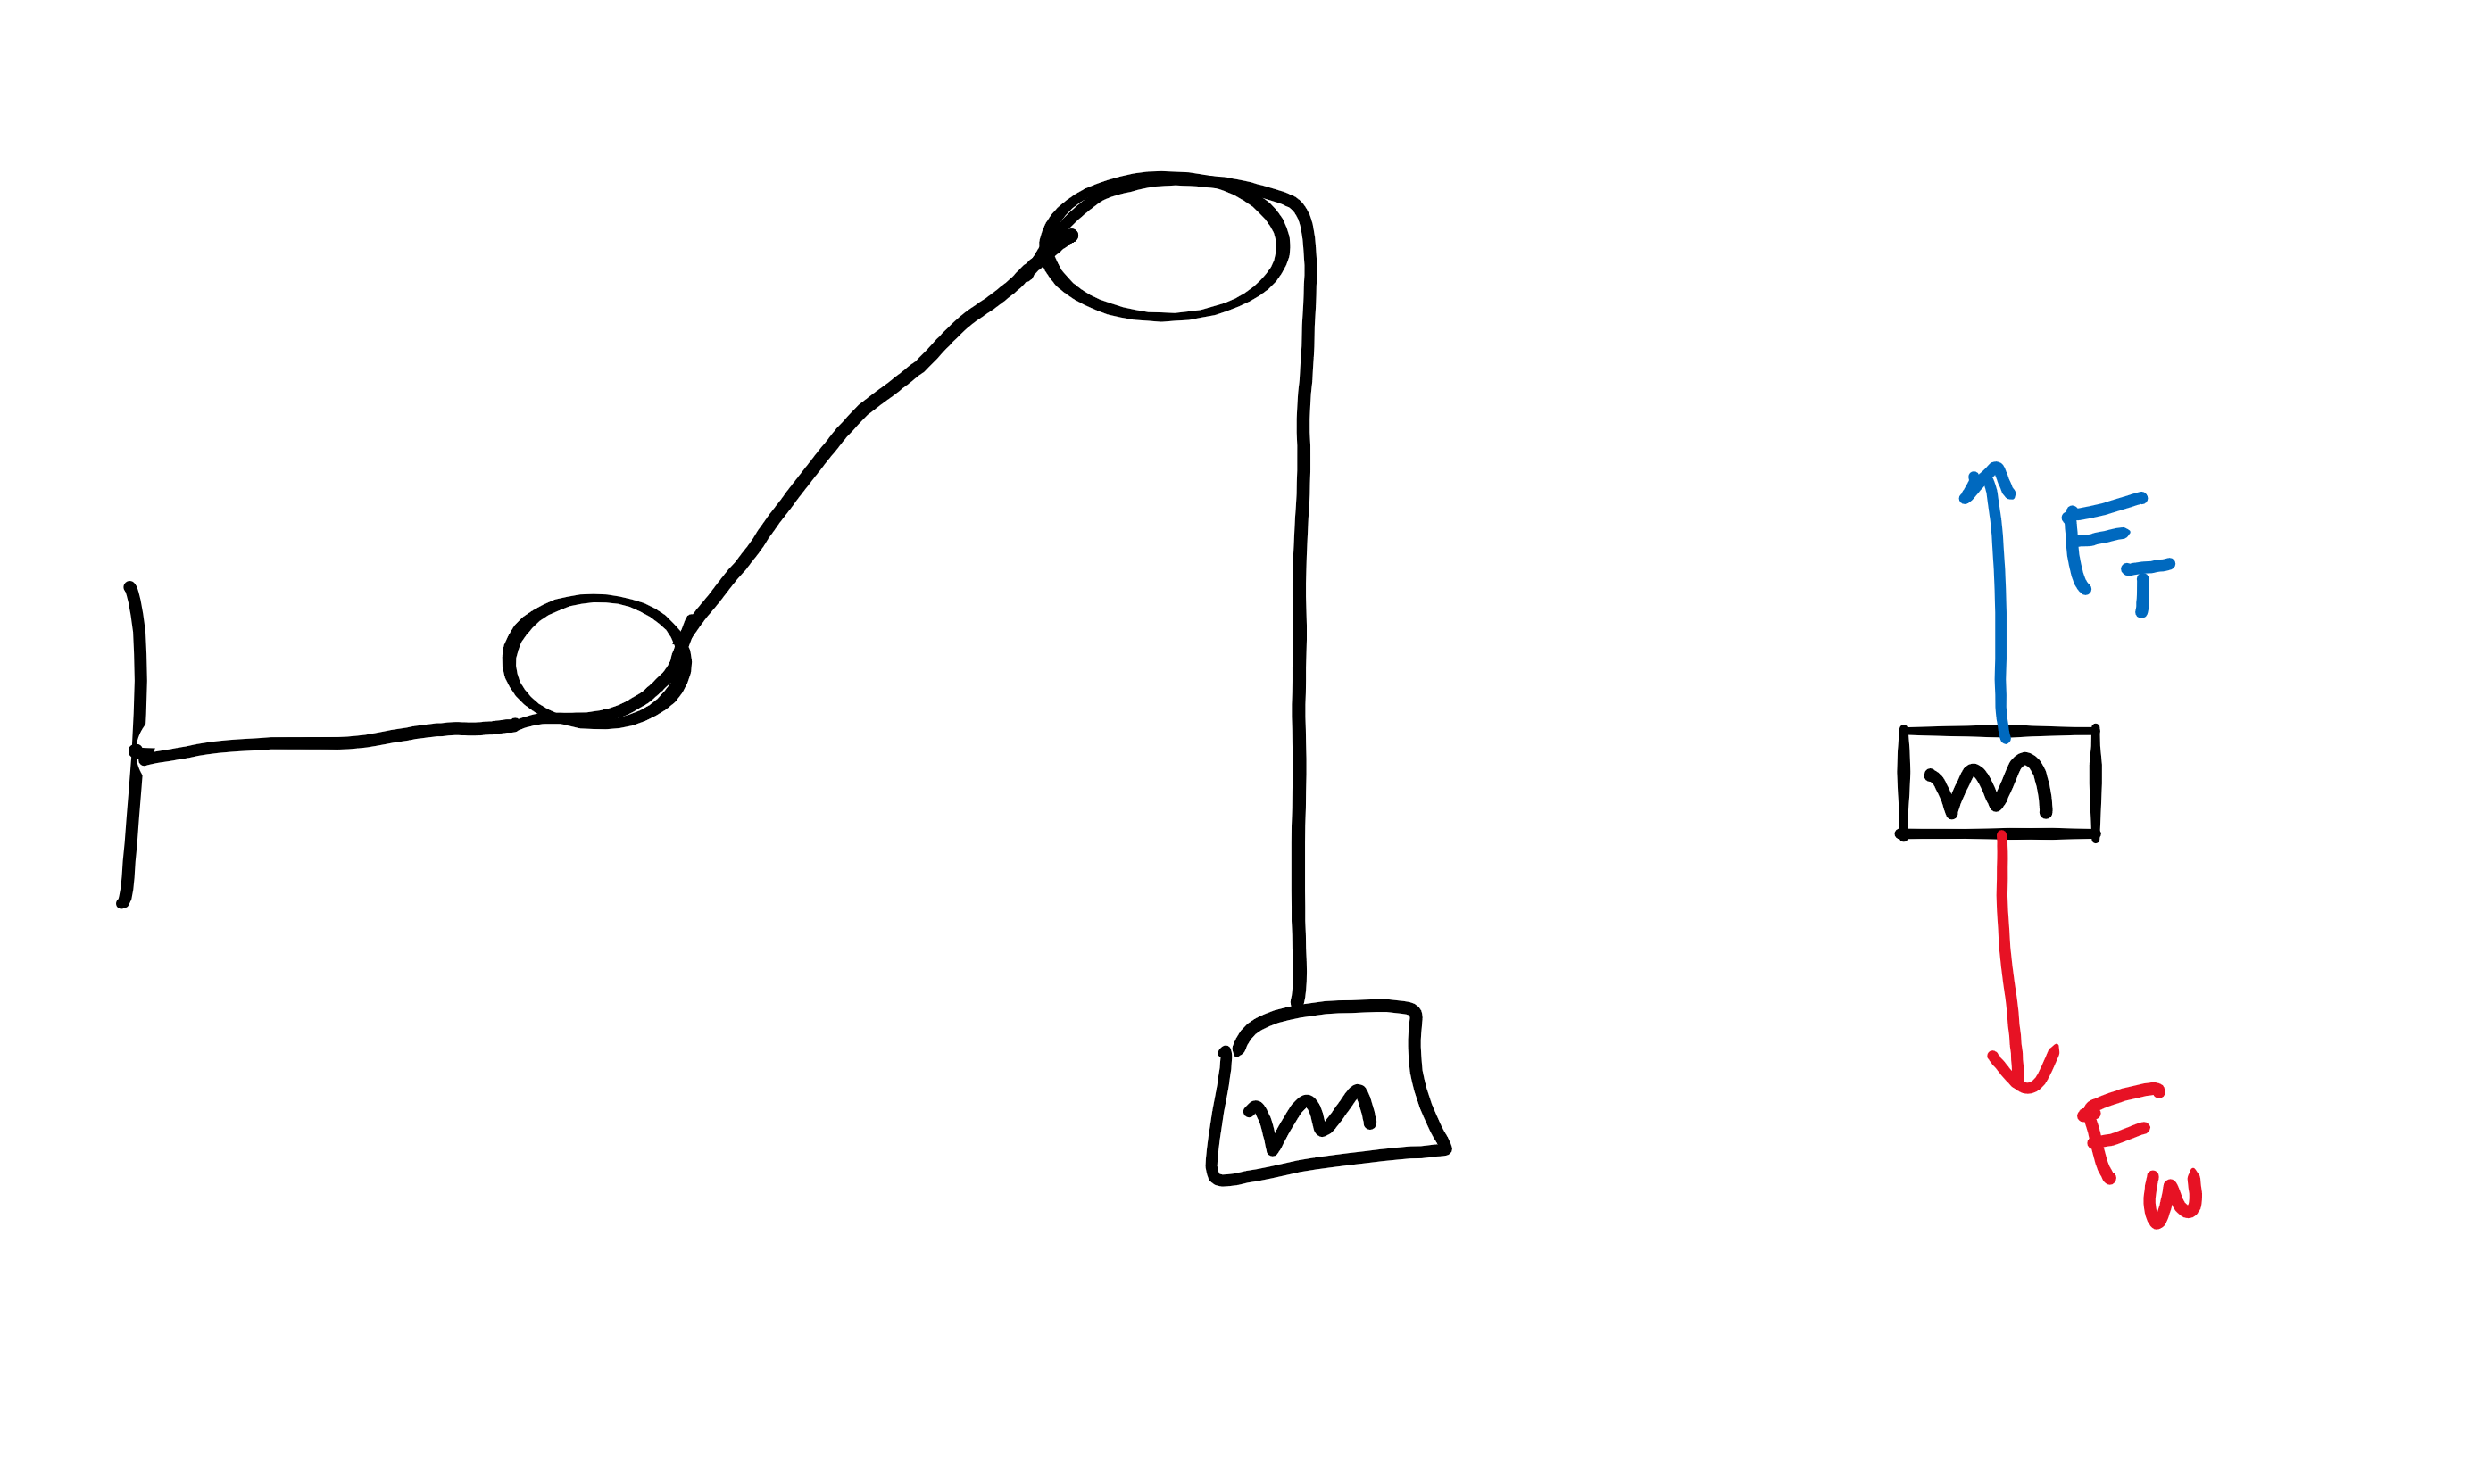
\includegraphics[width=0.5\textwidth]{chapters/ch3/images/fig3_3.PNG}
\end{center}

In the FBD pictured above, despite the rope changing direction multiple times across the pulley, it is still the same rope. Therefore, the tension force of the rope will be the same across the entire rope, and we can simply represent the tension force by one vector in the FBD. Algebraically solving this system results in the following:

$$
	\begin{aligned}
		&\sum F = m\vec{a} = 0 \:\:\:\text{(object is in equilibrium)}\\
		&\sum F_x = 0 \:\:\:\text{(there are no forces in the $x$ direction)}\\
		&\sum F_y = F_T - F_g = F_T - mg
	\end{aligned}
$$

\subsection*{On A Ramp}

Before drawing the FBD, it is important to note that the easiest way to solve this is to change your coordinate system to match your ramp/inclined plane. To do this, line the x-axis up with the ramp. By doing this, the acceleration is only facing in the direction of the ramp (VS having to find acceleration in both the $x$ and $y$ components and combining them together to find the magnitude).\newpage

The FBD looks like the following:

\begin{center}
	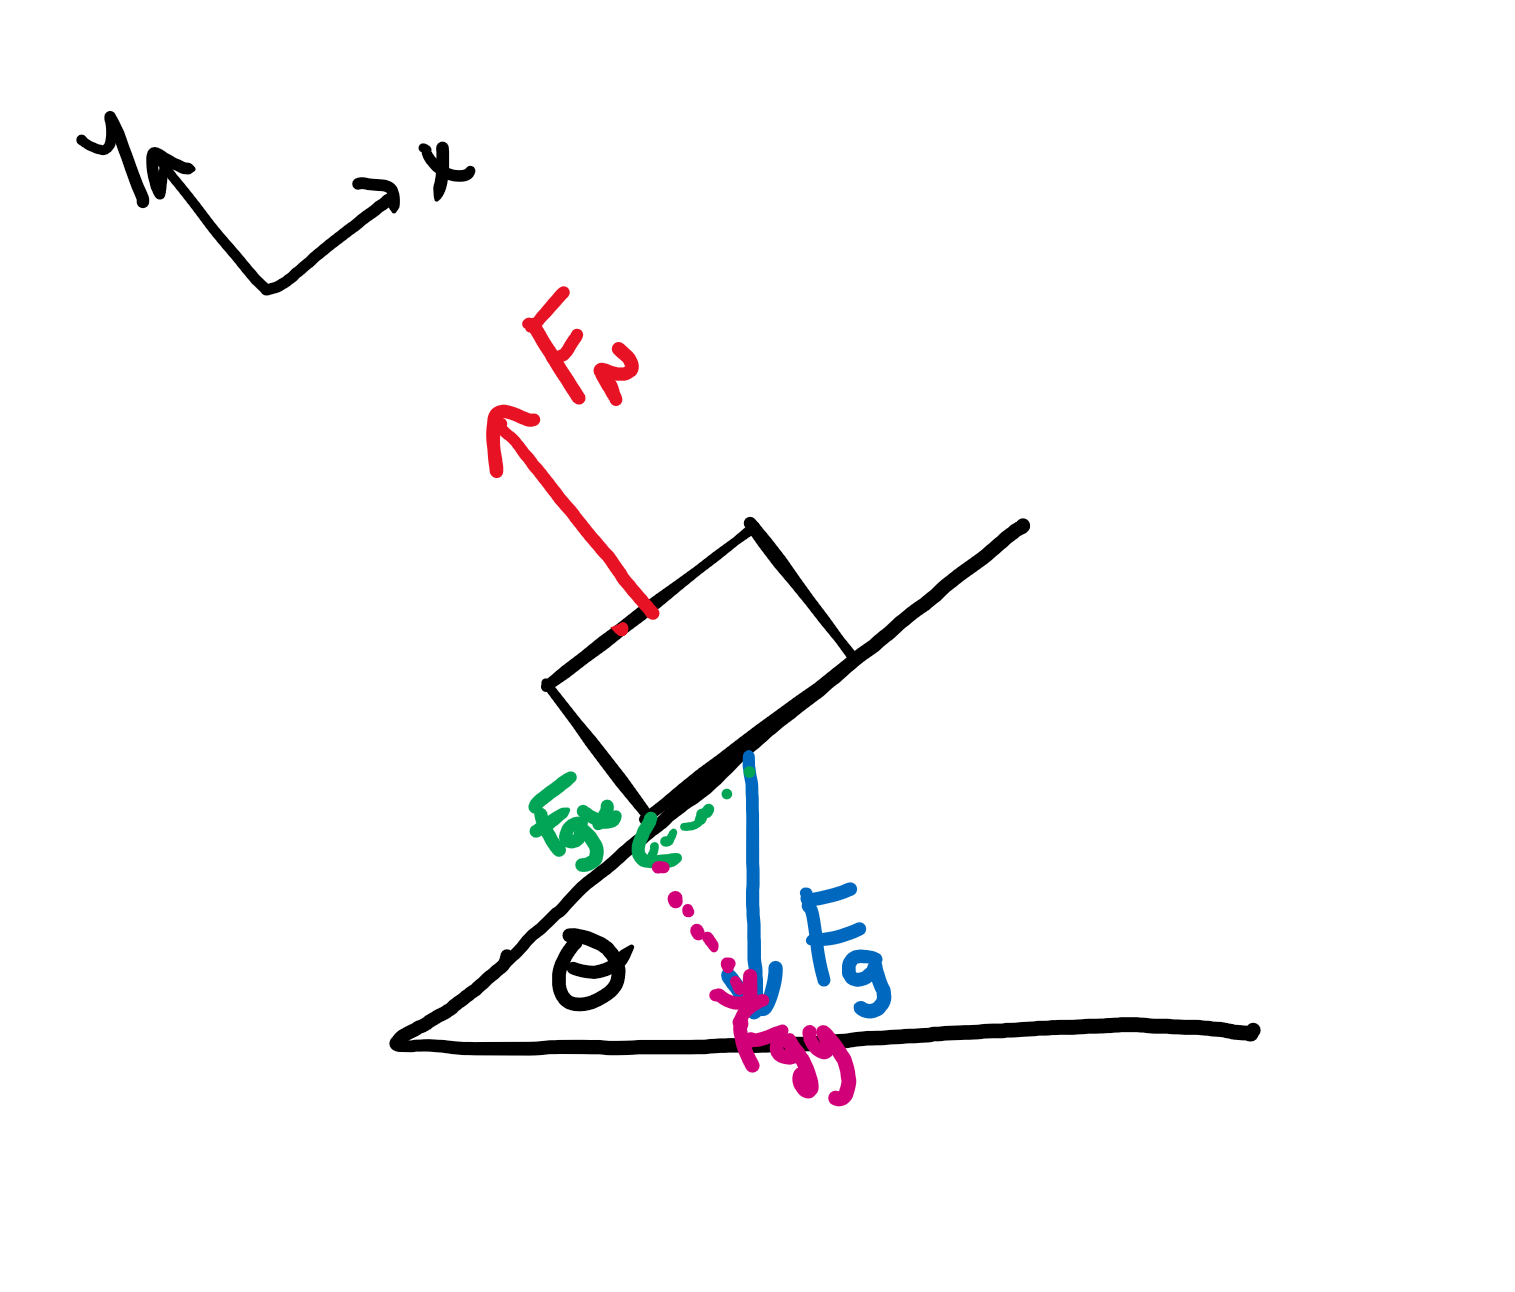
\includegraphics[width=0.5\textwidth]{chapters/ch3/images/fig3_4.PNG}
\end{center}

We can then solve this system algebraically:

$$
	\begin{aligned}
		&\sum \vec F = m\vec{a}\\
	\end{aligned}
$$

$$
	\begin{aligned}
		&\sum \vec F_x = -F_{gx}\\
		&-F_{gx} = m\vec{a}\\
		&-mg = m\vec{a}\\
		&\frac{-mg}{m} = \vec{a}\\
		&{-g} = \vec{a}
	\end{aligned}
$$

$$
	\begin{aligned}
		&\sum \vec F_y = 0 \:\:\: \text{(object is in equlibrium)}\\
		&F_{N} - F_{gy} = 0\\
		&F_N = F_{gy}
	\end{aligned}
$$
\newpage

\subsection*{Example Problems}

\begin{problem}
	A hockey puck experiences two forces, $\vec{F_1}$ and $\vec{F_2}$. Find the magnitude and angle of the acceleration of the hockey puck.

	\begin{center}
		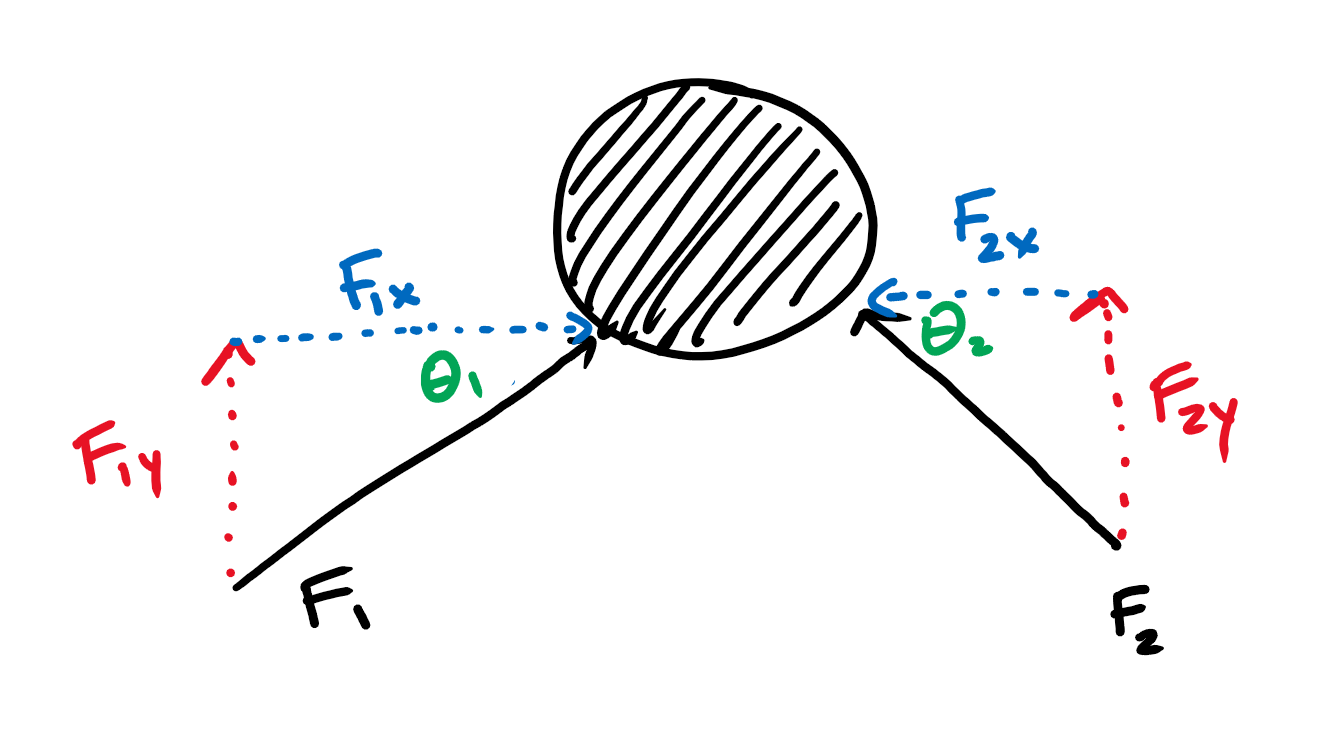
\includegraphics[width=0.5\textwidth]{chapters/ch3/images/fig3_5.PNG}
	\end{center}

	$$
		\begin{aligned}
			&\sum F_x = ma_x = F_1\cos\theta_1 - F_2cos\theta_2\\
			&\sum F_y = ma_y = F_1\sin\theta_1 + F_2\sin\theta_2\\
			&\vec a = a_x \vec i + a_y \vec j\\
			&|\vec a| = \sqrt{a_x^2 + a_y^2}\\
			&\phi = \arctan\left(\frac{a_y}{a_x}\right)
		\end{aligned}
	$$
\end{problem}



\begin{problem}
	A block of mass $m_1$ is attached to a pulley and sits on a slope with angle of inclination $\theta$. Two additional masses $m_2$ and $m_3$ are hanging off the side of the slope and are also attached to the pulley. All three masses are attached to the same string. Find the tension force and the acceleration of the third block.

	\begin{center}
		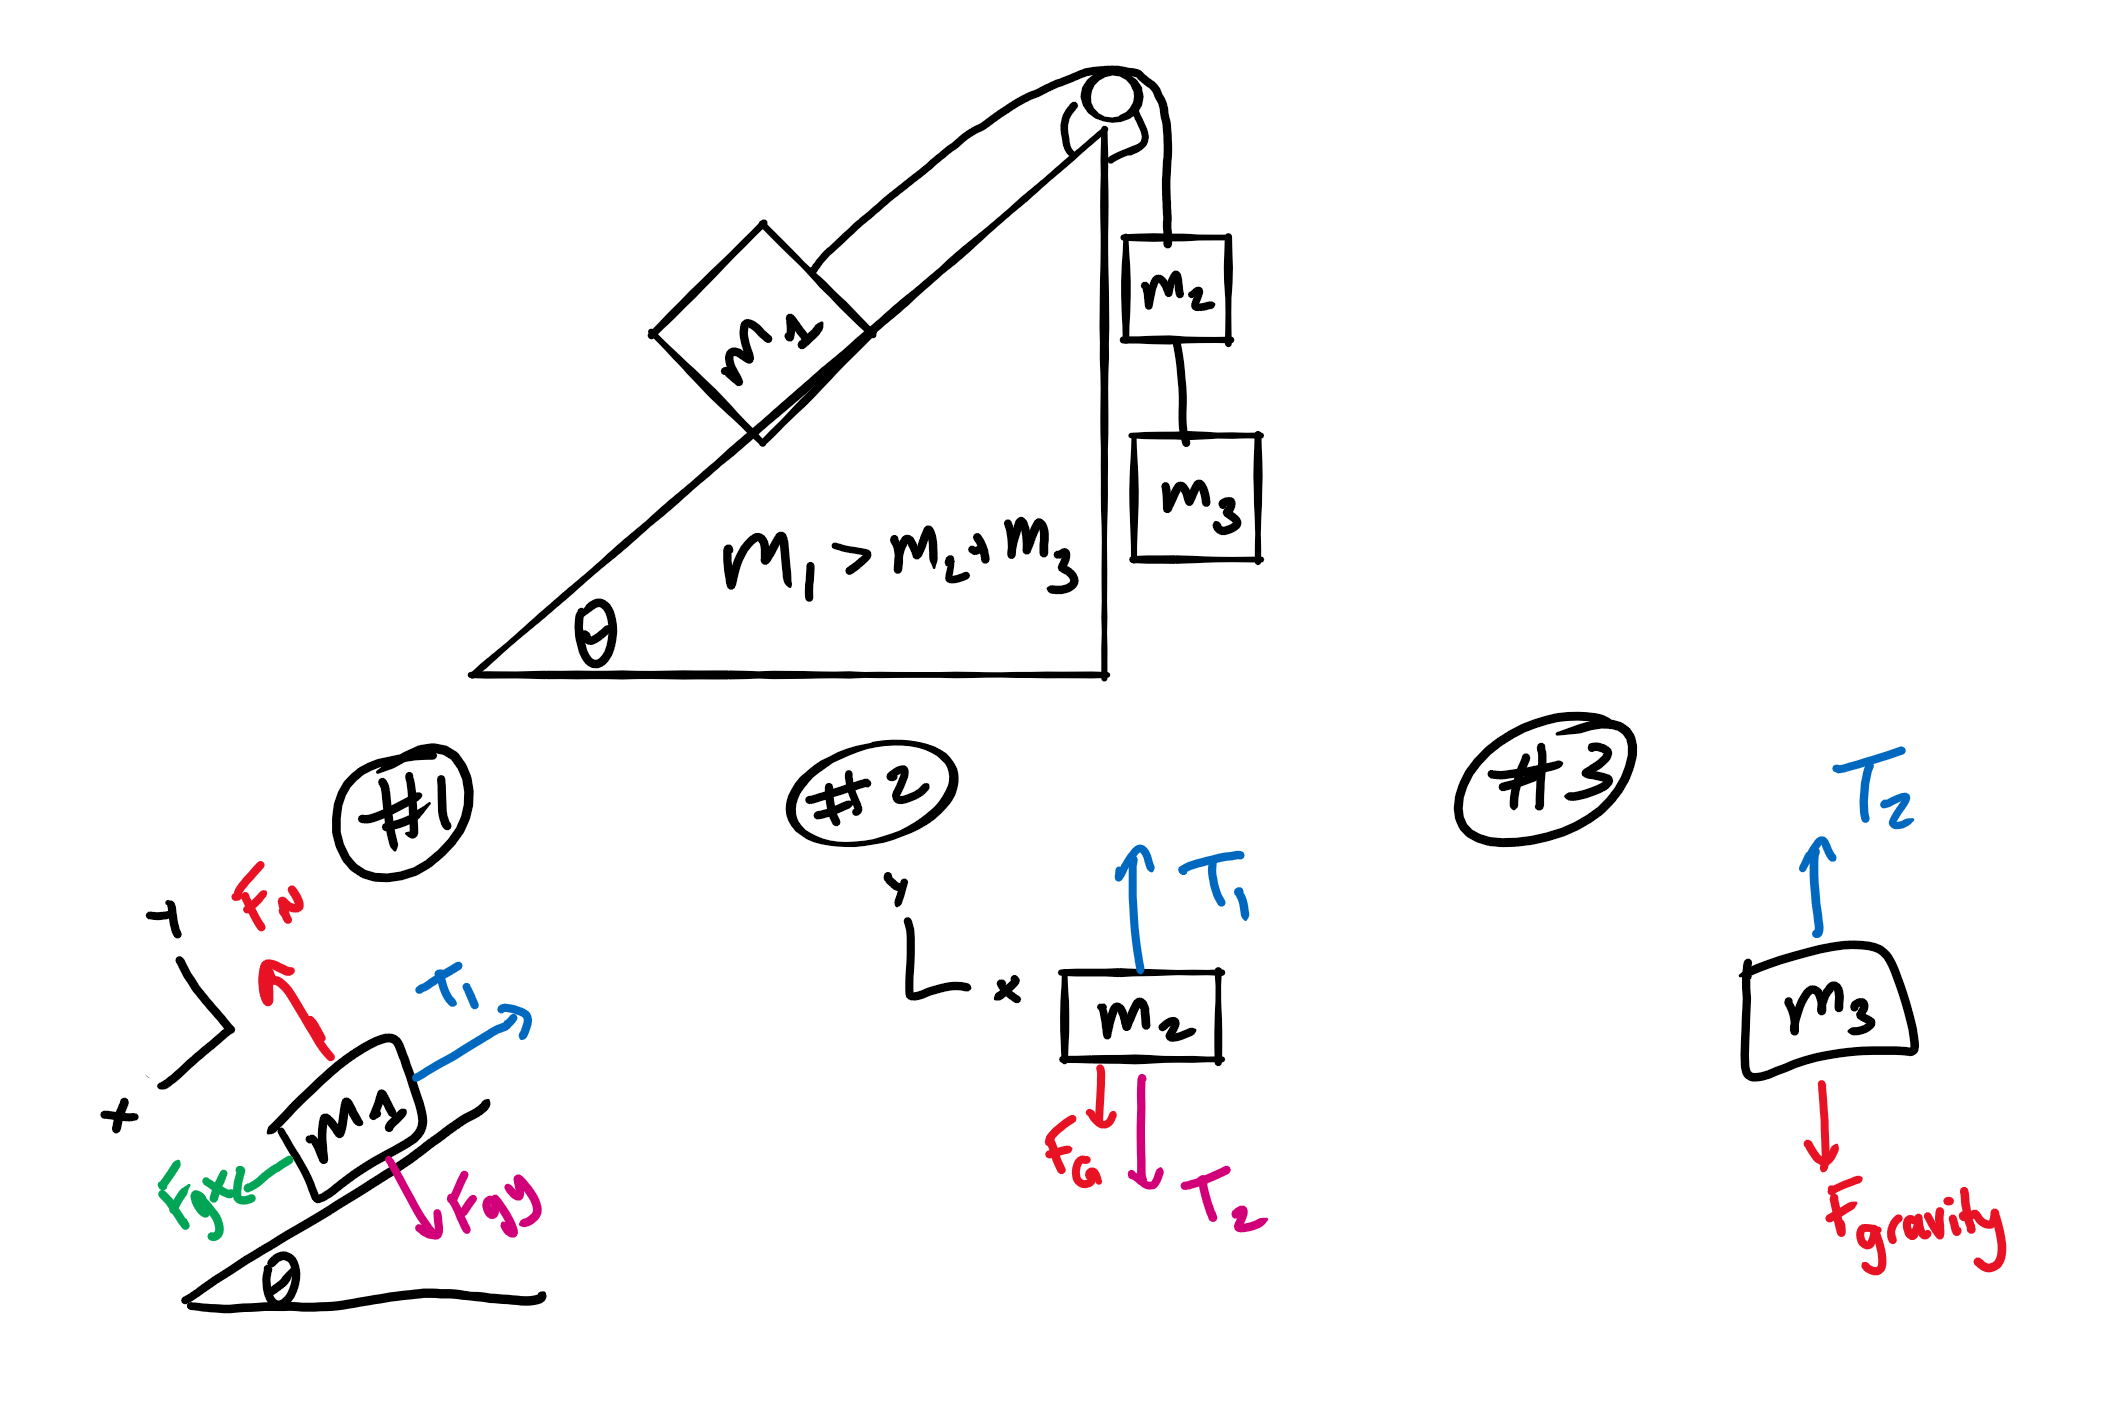
\includegraphics[width=0.5\textwidth]{chapters/ch3/images/fig3_6.PNG}
	\end{center}

	For \#1:
	$$
		\begin{aligned}
			\sum F_x = m_1a = m_1g\sin\theta - T_1\\
			\sum F_y = 0 = F_N - m_1g\sin\theta
		\end{aligned}
	$$

	For \#2:
	$$
		\begin{aligned}
			\sum F_y = m_2a = T_1 - T_2 - m_2g\\
		\end{aligned}
	$$


	For \#3:
	$$
		\begin{aligned}
			\sum F_y = m_3a = T_2 - m_3g
		\end{aligned}
	$$
\end{problem}



\section{Frictional Force}
	
	
\begin{definition}[Frictional Force]{def:label}
	There are two different types of frictional forces:

	\begin{itemize}
		\item \textbf{STATIC FRICTION:} A frictional force that is opposing the object when a force is applied to an object, but an object is not moving. The magnitude of this force \textit{changes with the magnitude of the force being applied}.
		
		$$F_{f} \le \mu_s F_N$$

		\textit{INSERT A GRAPH HERE}

		\item \textbf{KINETIC FRICTION:} A frictional force that opposes the object while the object is in motion. This force \textit{remains constant}.
		
		$$F_{f} = \mu_k F_N$$

		In all cases, $\mu$ is the coefficient of friction (which is a constant that varies depending on the surface that the object is on).\\

		Another thing to note is that $\mu_k < \mu_s < 1$.\\

		If the system is at rest or has no acceleration, use \textbf{static coefficient of friction}. If the system is accelerating, use the \textbf{kinetic coefficient of friction}.
	\end{itemize}
\end{definition}

\begin{problem}
	A car is traveling at a velocty of $1.6 \frac{\m}{\s}$ with a mass of 1500\kg \text{ }for a distance of 50\m. Assume that the acceleration is constant. Find the coeffeficient of kinetic friction. \\

	\begin{center}
		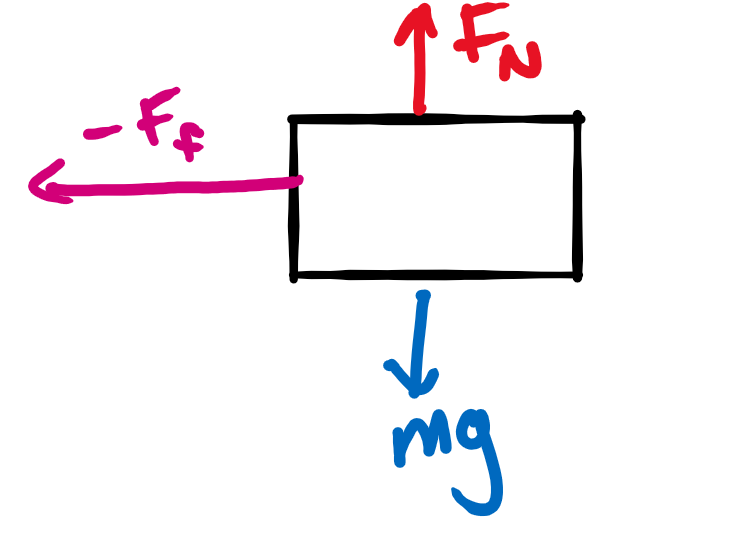
\includegraphics[width=0.5\textwidth]{chapters/ch3/images/fig3_8.PNG}
	\end{center}

	First, find the sum of the forces in the $y$-direction:
	$$
	\begin{aligned}
		&\sum F_y = 0\\
		&F_N - mg = 0\\
		&F_N = mg
	\end{aligned}
	$$

	Now, find the sum of the forces in the $x$-direction:
	$$
	\begin{aligned}
		&\sum F_y = ma\\
		&-F_f = ma\\
		&\mu_k F_N = ma\\
		&\mu_k mg = ma\\
		&\mu_k = -\frac{a}{g}
	\end{aligned}
	$$

	Using kinematics equations, we can solves for $a$:
	$$
	\begin{aligned}
		&v_f^2 = v_i^2 + 2a\Delta x\\
		&a = \frac{v_f^2-v_i^2}{2 \Delta x}\\
		&a = \frac{\left(0\frac{\m}{\s}\right)^2 - \left(1.\bar{6} \frac{\m}{\s}\right)^2}{2 \cdot 50 \m}\\
		&a = -7.7 \frac{\m}{\s^2}
	\end{aligned}
	$$

	Now, we can solve for $\mu_k$:
	$$
	\begin{aligned}
		&\mu_k = -\frac{a}{g}\\
		&\mu_k = -\frac{-7.7 \frac{\m}{\s^2}}{9.8 \frac{\m}{\s^2}}\\
		&\mu_k = \text{ANSWER}
	\end{aligned}
	$$
\end{problem}


\section{Air Drag}

\begin{definition}[Air Drag]{def:label}
	$$
		F_{AD} = \frac{1}{2}C\rho A|v|^2
	$$

	$C$ = coefficient of "air" friction\\
	$\rho$ = the density of the air\\
	$A$ = the cross-sectional area of the object\\
	$v$ = the velocity of the object (SCALAR QUANTITY)
\end{definition}
\newpage


\begin{problem}
	A bowling ball with mass of 5\kg \text{ }and radius of 4 cm falls through the air with a $C$ value of 1.2 and air density of 1.23 $\frac{\kg}{\m^3}$. What is the terminal velocity of the bowling ball?

	$$
	\begin{aligned}
		\sum F_y &= 0 = F_{AD} - mg\\
		F_{AD} &= mg\\
		\frac{1}{2}C\rho Av^2 &= mg\\
		v &= \sqrt{\frac{2mg}{C\rho A}}\\
		v &= \sqrt{\frac{2(5\kg)\left(9.81\frac{\m}{\s^2}\right)}{(1.2)\left(1.23 \frac{\kg}{\m^3}\right)(0.04\m)^2\pi}}\\
		v &\approx 115 \frac{\m}{\s^2}
	\end{aligned}
	$$
\end{problem}


\section{Centripetal Forces}

\begin{itemize}
	\item Recall that $a_{centripetal} = \frac{|v|^2}{R}$
	\item A \textbf{centripetal force} is any force that causes a system to begin rotating in a circle
	\item You would still use Newton's second law, but the acceleration used in Newton's Second Law will be the \textit{centripetal acceleration}
\end{itemize}


\begin{problem}
	You are riding on a ferris wheel and your mass is 50\kg. The radius of the ferris wheel is 25\m. You go around the ferris wheel at a rate of 1 revolution per minute. Find $F_N$ a) at the bottom of the ferris wheel and b) at the top of the ferris wheel.\\

	a) (top)

	$$
	\begin{aligned}
		\sum F_{T} &= ma_c = -N_{T} + mg\\
		m\left(\frac{|v|^2}{R}\right) &= -N_{T} + mg\\
		N_{T} &= mg - \frac{mv^2}{R}
	\end{aligned}
	$$

	b) (bottom)
	$$
	\begin{aligned}
		\sum F_{B} &= ma_c = N_B - mg\\
		N_B &= m\left(g + \frac{v^2}{R}\right)
	\end{aligned}
	$$
\end{problem}



\begin{problem}
	A car with masss $m$ is going around a turn on an inclined plane inclined at an angle $\theta$. \textbf{DRAW A FBD} and determine the friction force being applied.\\


	Sum of the forces in the $y$-direction:
	$$
	\begin{aligned}
		\sum F_y &= ma_y = F_N - mg\cos\theta\\
		\sum F_y &= ma\sin\theta = F_N - mg\cos\theta\\
		F_N &= m\left(\frac{v^2}{R}\sin\theta - g\cos\theta\right)
	\end{aligned}
	$$


	Sum of the forces in the $x$-direction:
	$$
	\begin{aligned}
		\sum F_x &= ma_x = F_f + mg\sin\theta\\
		\sum F_x &= ma\cos\theta = F_f + mg\sin\theta\\
		F_f &= m(a\cos\theta - g\sin\theta)\\
		F_f &= m\left(\frac{v^2}{R}\cos\theta - g\sin\theta\right)\\
		\mu F_N &= m\left(\frac{v^2}{R}\cos\theta - g\sin\theta\right)
	\end{aligned}
	$$

	\textbf{NOW GO BACK AND TRY THIS PROBLEM AGAIN BUT WITHOUT TILTING THE AXES AND PUT THIS INTO YOUR NOTES}
\end{problem}


\begin{problem}
	If the static coefficient of friction is 0.7, then how fast can a 5 m merry-go-round spin by your slide. 

	$$
	\begin{aligned}
		\sum F_y = 0 = F_N - mg\\
		F_N = mg
	\end{aligned}
	$$

	$$
	\begin{aligned}
		\sum F_x &= ma = F_f\\
		\mu_sF_N &= ma\\
		\mu_smg &= ma\\
		\mu_sg &= \frac{v^2}{R}\\
		v &= \sqrt{\mu_sgR}
	\end{aligned}
	$$
\end{problem}